As an alternative to metropolitan statistical areas (or Core Based Statistical Areas), many researchers use
Commuting Zones because they cover the entire country and group counties based on commuting flows, which is a
measure of labor market integration. However, few researchers are familiar with the methodology used to develop
these zones. To that end, this section describes the methodology used by Tolbert and Sizer (1996) in
developing the zones.\footnote{The methodology was originally used in Tolbert and Killian (1987), but the 1996
paper is much more widely cited, and the zones from that paper are the ones most commonly used.}

The Economic Research Service (ERS), an agency under the U.S. Department of Agriculture for which this
methodology was developed, distributes commuting zone definitions on its website. Commuting Zones are
especially relevant for the economic analysis of rural areas because they include all counties, not just urban
counties.

The methodology used by TS1996 has two important components: the dissimilarity matrix, which measures how ``far'' observations are from one another, and the clustering method, which decides how observations are divided into groups. The next two subsections outline how TS1996 address these two components.

\subsection{Dissimilarity Matrix}

The dissimilarity matrix (or conversely, similarity matrix) is a representation of the relative distance between pairs of counties, as measured by an entry in the matrix $D_{ij}$.\footnote{The clustering method used dictates using a dissimilarity or similarity matrix; one is just the complement of the other.} TS calculated the dissimilarity matrix $D$, where an entry $D_{ij}$ is the dissimilarity of county $i$ from county $j$, as below:

\begin{equation}\label{eqn:diss}
D_{ij} = 1- \frac{f_{ij}+f_{ji}}{min(rlf_{i},rlf_j)}
\end{equation}

In the above equation, $f_{ij}$ is the number of commuters who live in county $i$ and work in county $j$, and $rlf_i = \sum_j f_{ij}$ (including $f_{ii}$) is the measure of the resident labor force. TS1996 use the 1990 Journey-to-Work data, which tabulates the commuting information from the 1990 Census Long-form response.\footnote{Other releases of commuting zones have used 1980 and 2000 data. All three are available at \url{http://www.ers.usda.gov/data-products/commuting-zones-and-labor-market-areas.aspx}.}

\subsection{Clustering Method}

After constructing this dissimilarity matrix, TS1996 use it as an input into their clustering method. In general, clustering methods are used in data science to decide which observations are similar to one another, usually by dividing the observations into distinct groups. In their application, TS1996 use the average-linkage hierarchical clustering algorithm (PROC CLUSTER in SAS). The hierarchical clustering method uses the dissimilarity matrix in the following way. To begin, every county is its own cluster. Then, it finds the lowest value $D_{ij}$ in the dissimilarity matrix, and combines those two counties together. It then recalculates the dissimilarity values between the new cluster and all other clusters in the following way:\footnote{There are multiple distance measures that one can use for a clustering procedure; this is the measure used by TS1996.}

\begin{equation}
D_{KL} = \frac{1}{N_K N_L} \sum_{i \in C_k} \sum_{j \in C_L} D_{ij}
\end{equation}

Where $K$ and $L$ are clusters, and $D_{ij}$ is calculated as in Equation \ref{eqn:diss}.

This process continues until the researcher stops the process by choosing a ``cutoff'' height, $H$, such that if $D_{KL}>H$, then $K$ and $L$ do not merge.

We illustrate this process in Appendix Figure \ref{fig:caliclusters}, which shows the hierarchical progression of how counties are clustered together for California. In the top left-hand corner, only a few counties have joined at a height of $H=0.8$. As we increase the height from 0.8 to 0.88, more counties are joined together, which is also true when the height is 0.96. Finally, at a height of 1, almost all the counties have merged together, forming one large cluster and a few much smaller clusters.

\subsection{Our Replication}
\FloatBarrier

In order to replicate the clustering result in TS1996, which we  refer to as FKV1990, we use the 1990 Census JTW data and the methodology described above, with one important exception. Because of computing power constraints in 1996, TS1996 divided the country into six overlapping regions and performed the clustering algorithm on each region separately, and then manually resolved conflicts in overlapping regions. This decision has two consequences for users: first, the height cutoffs across regions are not the same, because there is a normalization step before the algorithm merges observations. Second, it induces some subjectivity, since there are likely conflicts in cluster assignment in areas with overlapping regions.

Rather than follow their methodology and divide the country into regions, we run the hierarchical clustering algorithm on the entire country, and use the height cutoff that most closely replicates their original zones, which we find to be 0.9418. TS1996's zones and our replication are in Figure \ref{fig:czreplication}, and our summary statistics comparing the zones are in Table \ref{tab:replication}.

While our replication does not perfectly match their zones, this is not surprising, because we did not split the country into overlapping regions. With that caveat, our replication matches the moments from the commuting zones closely, and for a given county, about 80\% of the counties in our new zones match with the counties in the original zones.
\begin{figure}[tbh]\centering
\begin{tabular}{cc}
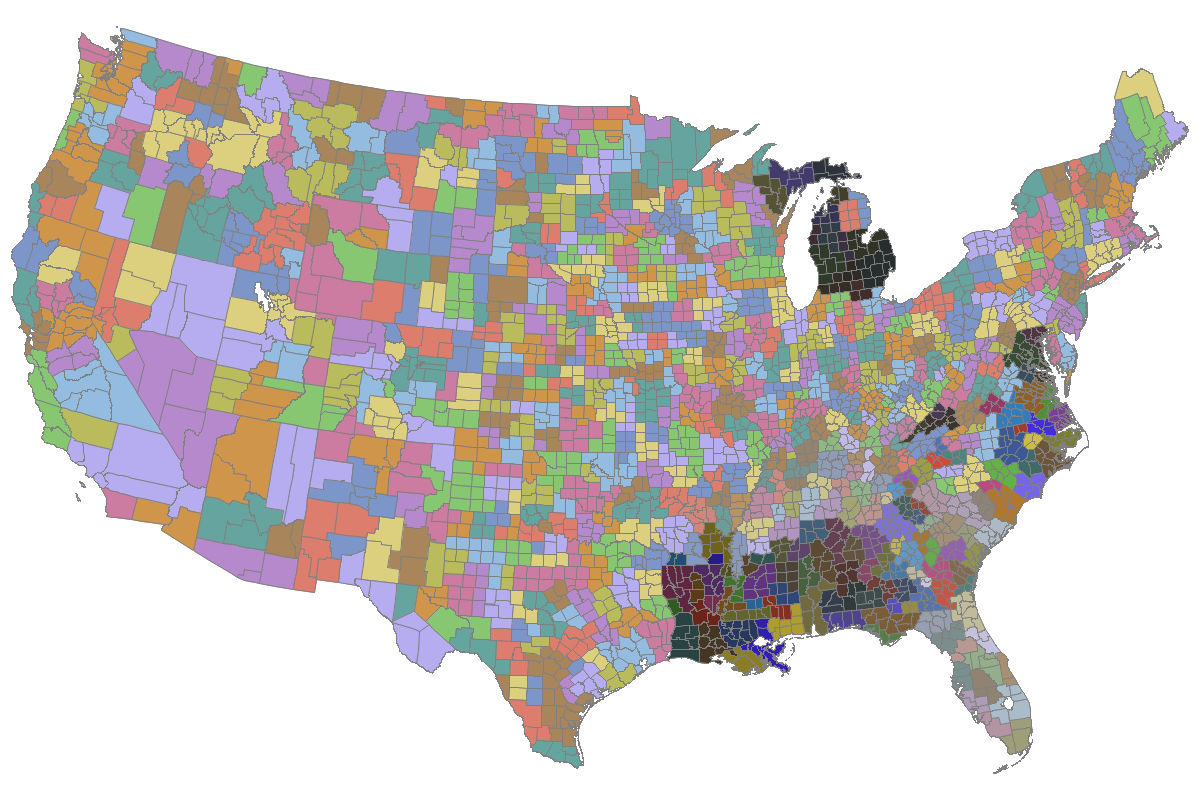
\includegraphics[scale=0.25]{./figures/commutingzones.png}&
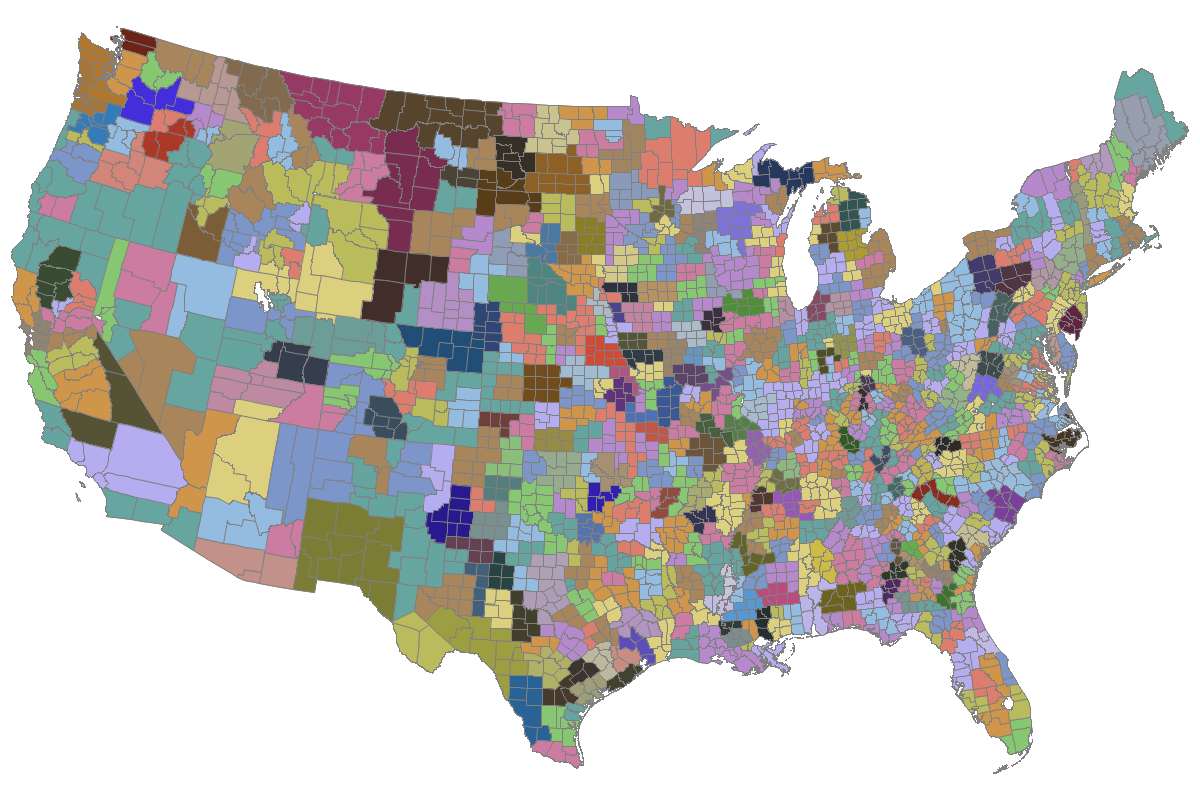
\includegraphics[scale=0.25]{./figures/clustermap_jtw1990_x.png}\\
Commuting Zones from TS1996 & Replication of Commuting Zones \\
\end{tabular}
\caption{Replication of Commuting Zones from TS1996: County Mapping \label{fig:czreplication}}
\end{figure}

% source: name of SAS program
% Last updated:

\begin{table}\centering
\caption{Replication of Commuting Zones from TS1996: Summary Statistics \label{tab:replication}}
\begin{tabular}{lcc}
\hline\hline
       & TS1990 &  FKV1990  \\
       \hline
Mean Cluster Size &  4.24  & 4.19 \\
Median Cluster Size & 4 & 4 \\
Number of Clusters & 741 & 741  \\
Number of Singletons & 62 &  10 \\
\hline
\multicolumn{3}{p{4in}}{\footnotesize \textit{Notes}: Both TS1990 and FKV1990 are based on JTW tabulations from the 1990 Census. Summary statistics for TS1990 are from Table 8 of TS1996.}\\
\end{tabular}
\end{table}


%Mark will look at writing a more efficient macro for this
